%include part: see main.beamer.tex and main.article.tex
%include common packages and settings
\usepackage{etex} %эта магическая херь избавляет от переполнения регистров TeX а!!!

\mode<article>{\usepackage{fullpage}}
\mode<presentation>{
    \usetheme{Madrid} %%Boadilla,Madrid,AnnArbor,CambridgeUS,Malmoe,Singapore,Berlin
    \useoutertheme{shadow}
} 

\usepackage[utf8]{inputenc}
\usepackage[russian]{babel}
\usepackage{indentfirst}
\usepackage{graphicx}

\usepackage{amsmath}
\usepackage{amsfonts}
\usepackage{amsthm}
\usepackage{algorithm}
\usepackage{algorithmic}

\usepackage[all]{xy}

\date{Лекция по дисциплине <<дискретная математика>>\\(\today)}
\author[М.~М.~Шихов]{Михаил Шихов \\ \texttt{\underline{m.m.shihov@gmail.com}}}

%для рисования графов пакетом xy-pic
\entrymodifiers={++[o][F-]}

%для псевдокода алгоритмов (algorithm,algorithmic)
\renewcommand{\algorithmicrequire}{\textbf{Вход:}}
\renewcommand{\algorithmicensure}{\textbf{Выход:}}
\renewcommand{\algorithmiccomment}[1]{// #1}
\floatname{algorithm}{Псевдокод}



\title{Нечёткие множества}


\begin{document}

%титул и содержание статьи
\mode<article>{\maketitle\tableofcontents}

%титул и содержание презентации
\frame<presentation>{\titlepage}
\begin{frame}<presentation>
    \frametitle{Содержание}
    \tableofcontents
\end{frame}

Нечеткие множества нашли широкое применение в области искусственного интеллекта и управления. Действительно, в этих областях весьма часто требуется задавать некоторые логические правила (отражающие знания или определяющие поведение объекта управления). Элементами этих правил могут являться весьма <<нечёткие>> понятия\ldots Допустим, что <<умная>> компьютерная система управления теплицей руководствуется следующими правилами, снимая показания температуры \verb"t" с датчика над кустом томатов:

\begin{frame}[fragile]
    \frametitle{Система контроля климата в теплице}
    \framesubtitle{Выращиваются томаты}
    
\begin{semiverbatim}
\alert{Если} t холодно,    \alert{то}
        включить_отопитель,
        выключить_охладитель;
    
\alert{Если} t оптимально, \alert{то}
        ничего_не_делать;
    
\alert{Если} t жарко,      \alert{то}
        выключить_отопитель,
        включить_охладитель;
\end{semiverbatim}
\end{frame}

В данных правилах используются следующие качественные описания температуры: \verb"холодно", \verb"оптимально", \verb"жарко". И, пожалуй, эти правила управления нас устроят, если мы на место томатов посадим пальму. Но пальму они не устроят, потому что то, что для томатов \verb"оптимально" (не говоря о \verb"холодно"), то пальме --- смерть! Очевидно, что под \verb"холодно", \verb"оптимально", \verb"жарко" понимаются некоторые множества --- диапазоны температур. Пойдя навстречу пальме, попытаемся изменить эти множества. Но мы столкнемся с некоторыми трудностями: 

\begin{frame}[fragile]
    \frametitle{Трудности получения знаний}
    \framesubtitle{Адаптация правил под пальму}
    
    \begin{tabular}{rl}
        \alert{Эксперт:}    & 22 градуса по цельсию --- для Вас \verb"оптимально"?\\
        \alert{Пальма:}     & Близко к оптимальному, да\ldots Но уже чуток холодновато\ldots \\
        \alert{Эксперт:}    & Значит \verb"холодно"?\\
        \alert{Пальма:}     & Нет, нет, не холодно, ну, может чуток\ldots \\
        \alert{Эксперт:}    & Значит все же \verb"оптимально"?\\
        \alert{Пальма:}     & Процентов на 90, я думаю\ldots\\
        \alert{Эксперт:}    & ммм\ldots
    \end{tabular}
\end{frame}

Вот тут и пригодятся нечеткие множества. Понятие нечетких множеств было введено Л.~Заде в 1965 году. Изложение  математических основ можно найти, например, в \cite{bib:gorbatovs:discrmath} или в прикладном контексте\footnote{Данная книга посвящена нейронным сетям --- важной области искусственного интеллекта} в \cite{bib:osovsky:neyro}. Краткая теория приведена ниже.


\section{Основные определения}


\subsection{Функция принадлежности}

Множество $A$, являющееся подмножеством некоторого универсального множества $U$, можно задать с помощью \emph{характеристической функции} (\emph{функции принадлежности}), определенной следующим образом для каждого $x\in U$:
\begin{frame}
    \frametitle{$A\subseteq\mathbb{U}$}
    \framesubtitle{Характеристическая функция $\mu_A:\mathbb{U}\to\{0,1\}$}
    
    \[
        \mu_A(x)=
        \begin{cases}
            1, &\text{если $x\in A$},\\
            0, &\text{в противном случае.}
        \end{cases}
    \]
\end{frame}

Итак, если для некоторого $x\in U$ функция $\mu_A(x)=1$, то $x$ принадлежит множеству $A$, если $\mu_A(x)=0$, то $x$ множеству $A$ не принадлежит. Для \emph{нечеткого} множества $A$ характерно то, что $\mu_A(x)$ принимает значение из отрезка $[0,1]$. 

\begin{frame}
    \frametitle{Нечёткое множество $A\subseteq\mathbb{U}$}
    \framesubtitle{Характеристическая функция $\mu_A:\mathbb{U}\to[0,1]$}
    
    \[
        A=\{x/\mu_A(x)|x\in U\}.
    \]
    
    \begin{definition}
        Значение $\mu_A(x)$ называется \alert{коэффициентом принадлежности}\footnote{То есть $\mu_A(x)$ определяет \alert{степень} принадлежности элемента $x\in\mathbb{U}$ множеству $A$. Если $\mu_A(x)>\mu_A(y)$, то элемент $x$ принадлежит множеству $A$ в большей степени, чем $y$} элемента $x$ множеству $A$.
    \end{definition}
\end{frame}




\begin{frame}
    \frametitle{Не вероятность!!!}
    
    \begin{example}[Нечеткое множество <<большой>> на универсуме <<животные>> для попугая] 
        \[
            \begin{split}
                \text{большой}=\{
                    \text{попугай}/1,\text{жираф}/0.98,\text{слон}/0.9,\\
                    \text{удав}/0.5,\text{зебра}/0.4,\text{гиена}/0.3,\\
                    \text{мартышка}/0.2,\text{клоп}/0.01,\text{кит}/0\}.
            \end{split}
        \]
        \qed
    \end{example}
    Как видно, коэффициенты $\mu_{\text{большой}}(x)$ сильно зависят от опыта <<эксперта>>: например, можно сказать, что попугай ни разу в жизни не видел кита. В этом отличие коэффициента принадлежности от, например, вероятности, с которой его часто путают.
\end{frame}


\subsection{Бесконечное нечёткое множество}

Когда универсальное множество $U$ бесконечно(счетно или континуально), то для того, чтобы задать $\mu_A(x)$ часто используют следующего вида аналитические функции (см. рис. \ref{fig:fuz:fuzzyTemperature}): 

\begin{frame}
    \frametitle{Аналитические функции принадлежности}
    
    \begin{itemize}
        \item сигмоидальные:
        \[
            \mu_A(x)=\frac{1}{1+\exp\left[-a(x-c)\right]},\mu_A(x)=\frac{x-c}{2(a+|x-c|)}+\frac{1}{2};
        \]
        
        \item гауссовские:
        \[
            \mu_A(x)=\exp\left[-\left(\frac{x-c}{d}\right)^{2b}\right],
            \mu_A(x)=\frac{1}{1+\left(\frac{x-c}{d}\right)^{2b}};
        \]
    \end{itemize}
\end{frame}

иногда используют фрагменты линейных функций, определенных на соответствующих интервалах (см. например, рис. \ref{fig:fuz:fuzzyOperations}).

\begin{frame}
    \frametitle{Аналитические функции принадлежности}
    
    \begin{figure}[!ht]
        \centering
        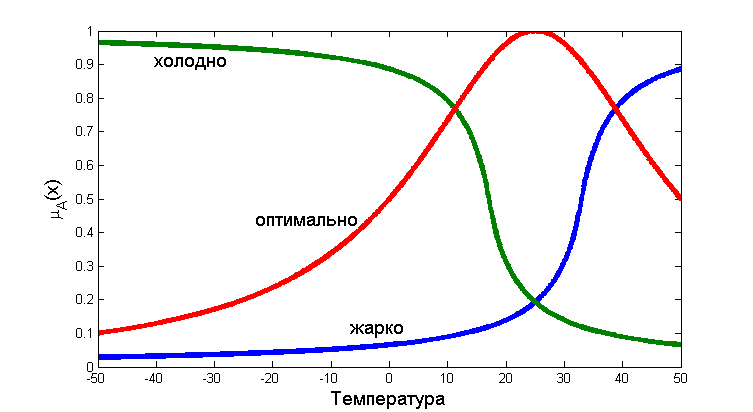
\includegraphics[width=0.8\textwidth]{fig/fuzzyTemperature}
        \caption{Аналитически заданные функции $\mu_A(x)$ для градаций температуры}
        \label{fig:fuz:fuzzyTemperature}
    \end{figure} 
\end{frame}


\section{Нечёткая логика}


\subsection{Операции над нечёткими множествами}

Над нечеткими множествами $A,B$ выделяют следующие основные операции:

\begin{frame}
    \frametitle{Операции над нечёткими множествами}
    
    \begin{enumerate}
        \item Объединение $A\cup B$: $\mu_{A\cup B}(x)=\max[\mu_A(x),\mu_B(x)]$;
        \item Пересечение $A\cap B$: $\mu_{A\cap B}(x)=\min[\mu_A(x),\mu_B(x)]$
        \item Отрицание $\overline{A}$: $\mu_{\overline{A}}(x)=1-\mu_A(x)$;
        \item Вычитание $A\backslash B$: $\mu_{A\backslash B}(x)=\min[\mu_A(x), 1-\mu_B(x)]$;
        \item Концентрация $CON(A)$: $\mu_{CON(A)}(x)=[\mu_A(x)]^2$;
        \item Растяжение $DIL(A)$: $\mu_{DIL(A)}(x)=\sqrt{\mu_A(x)}$;
        \item Нормализация $NORM(A)$: $\mu_{NORM(A)}(x)=\frac{\mu_A(x)}{\sup\{\mu_A(y)|y\in U\}}$;
    \end{enumerate}
    
    Особенности:
    \begin{itemize}
        \item $A\cup\overline{A}\neq \mathbb{U}$;
        \item $A\cap\overline{A}\neq\emptyset$.
    \end{itemize}
\end{frame}


$A\subseteq B$, если $\forall x\in U (\mu_A(x)\leq\mu_B(x))$. Для равенства: $A=B\Leftrightarrow (A\subseteq B)\land(B\subseteq A)$.


\subsection{Логические связки лингвистических переменных}

\begin{frame}
    \frametitle{Нечёткая логика}
    
    \begin{definition}
        В нечёткой логике нечеткому множеству ставится в соответствие качественное понятие --- \alert{лингвистическая переменная}. 
    \end{definition}
    
    Логическим связкам между лингвистическими переменными сопоставляются операции над соответствующими нечёткими множествам.
    \begin{center}
        \begin{tabular}{r|l}
            \hline\hline 
            Связка          & Операция    \\  \hline\hline 
            ИЛИ             & объединение   \\
            И               & пересечение   \\
            НЕ              & отрицание     \\
            ОЧЕНЬ           & концентрация  \\
            ПОЧТИ,ПРИМЕРНО  & растяжение    \\
            \hline
        \end{tabular}
    \end{center}
\end{frame}


\begin{frame}
    \frametitle{Концентрация (ОЧЕНЬ) и растяжение (ПРИМЕРНО)}
    
    \begin{figure}[!ht]
        \centering
        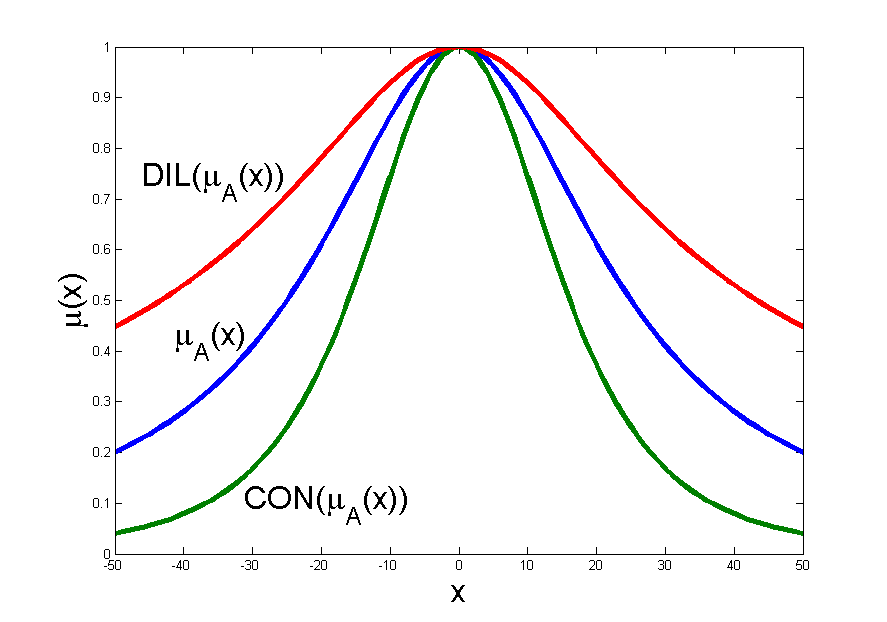
\includegraphics[width=0.7\textwidth]{fig/fuzzyConDil}
        \caption{Концентарция и растяжение нечёткого множества $A$}
        \label{fig:fuz:fuzzyConDil}
    \end{figure} 
\end{frame}

\begin{frame}
    \frametitle{Нечёткая логика}
    
    \begin{figure}
        \centering
        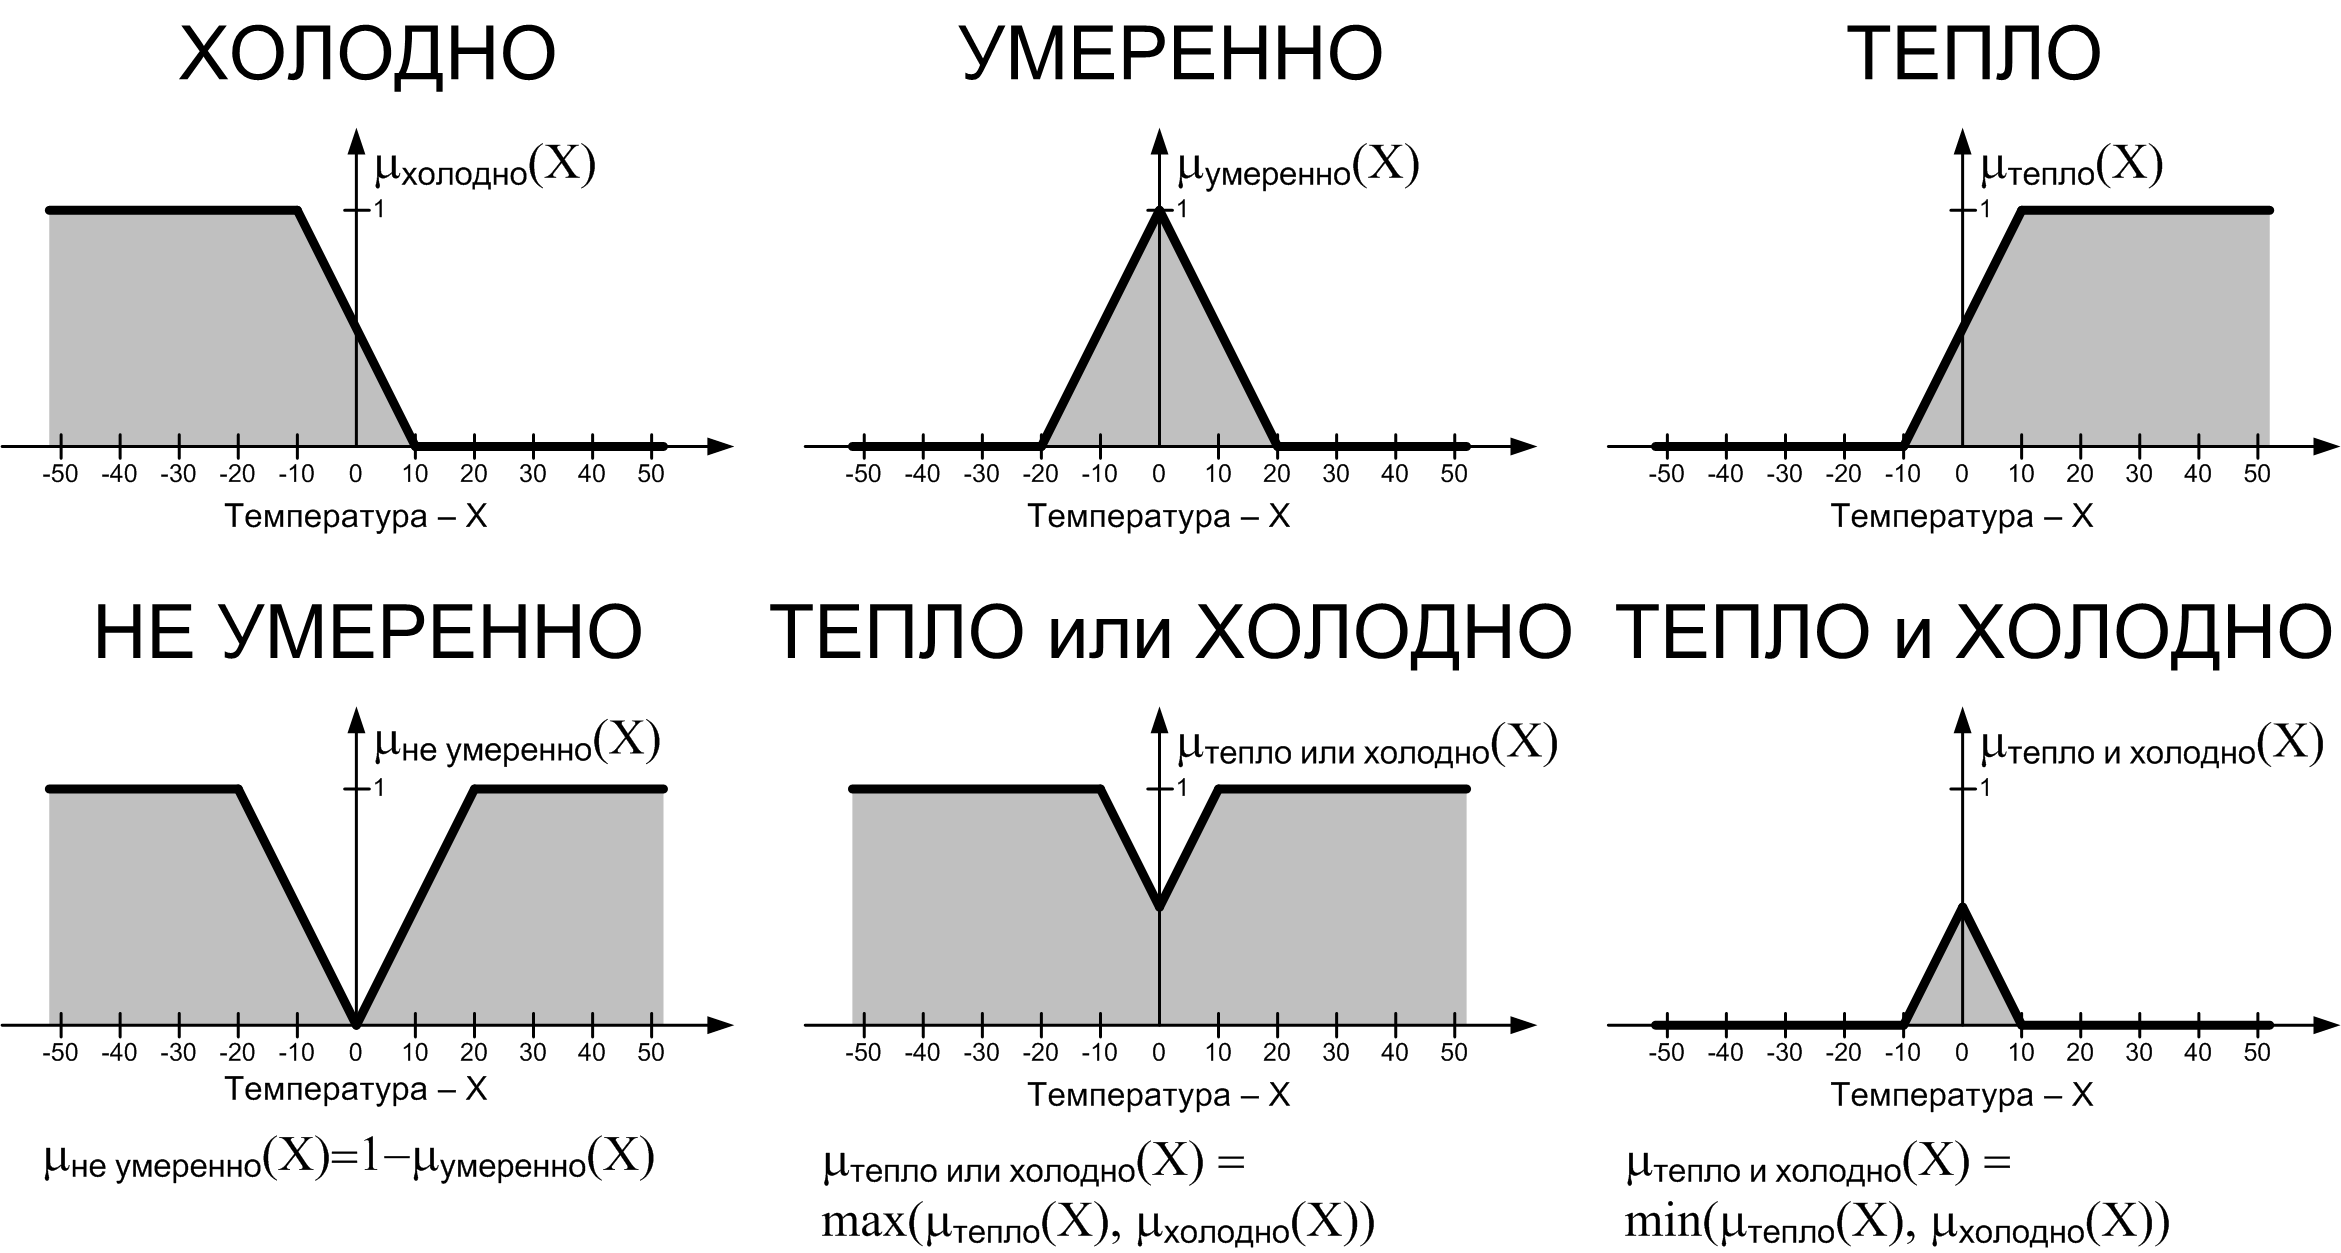
\includegraphics[width=0.9\textwidth]{fig/fuzzyOperations}
        \caption{Логические связки между лингвистическими переменными соответствуют операциям над нечеткими множествами}
        \label{fig:fuz:fuzzyOperations}
    \end{figure} 
\end{frame}


Видно, что бинарные операции основаны на функциях $\min$ и $\max$. В общем случае вместо $\min$ используют функцию $T:[0,1]\times[0,1]\to[0,1]$, которая называется \emph{$t$-нормой}, а вместо $\max$ используют функцию $S:[0,1]\times[0,1]\to[0,1]$, которая называется \emph{$t$-конормой}. $t$-норма обладает следующими свойствами:

\begin{frame}
    \frametitle{$t$-норма}
    \framesubtitle{$T:[0,1]\times[0,1]\to[0,1]$. Используется вместо $\min$}
    
    Свойства:
    \begin{enumerate}
        \item ограниченность: $T(0,0)=0,T(1,\mu)=\mu,T(\mu,1)=\mu$;
        \item монотонность: $T(\mu_1,\mu_2)\leq T(\mu_3,\mu_4)$, если $\mu_1\leq\mu_3, \mu_2\leq\mu_4$;
        \item коммутативность: $T(\mu_1,\mu_2)=T(\mu_2,\mu_2)$;
        \item ассоциативность: $T(\mu_1,T(\mu_2, \mu_3))=T(T(\mu_1,\mu_2),\mu_3)$;
    \end{enumerate}
    
    Примеры:
    \begin{itemize}
        \item $T(\mu_1,\mu_2)=\min(\mu_1,\mu_2)$;
        \item $T(\mu_1,\mu_2)=\mu_1\cdot \mu_2$;
        \item $T(\mu_1,\mu_2)=\max[0,\mu_1+\mu_2-1]$.
    \end{itemize}
\end{frame}

\begin{frame}
    \frametitle{$t$-конорма}
    \framesubtitle{$S:[0,1]\times[0,1]\to[0,1]$. Используется вместо $\max$}
    
    Свойства:
    \begin{enumerate}
        \item ограниченность: $S(1,1)=1,S(0,\mu)=\mu,S(\mu,0)=\mu$;
        \item монотонность: $S(\mu_1,\mu_2)\geq S(\mu_3,\mu_4)$, если $\mu_1\geq\mu_3, \mu_2\geq\mu_4$;
        \item коммутативность: $S(\mu_1,\mu_2)=S(\mu_2,\mu_2)$;
        \item ассоциативность: $S(\mu_1,S(\mu_2, \mu_3))=S(S(\mu_1,\mu_2),\mu_3)$;
    \end{enumerate}
    
    Примеры:
    \begin{itemize}
        \item $S(\mu_1,\mu_2)=\max(\mu_1,\mu_2)$;
        \item $S(\mu_1,\mu_2)=\mu_1+\mu_2-\mu_1\cdot\mu_2$;
        \item $S(\mu_1,\mu_2)=\min[1,\mu_1+\mu_2]$.
    \end{itemize}
\end{frame}


\appendix


\begin{frame}
    \frametitle{В заключение}
    
    Понятие нечетких множеств было введено Л.~Заде в 1965 году. Изложение  математических основ можно найти, например, в \cite{bib:gorbatovs:discrmath} или в прикладном контексте\footnote{Данная книга посвящена нейронным сетям --- важной области искусственного интеллекта} в \cite{bib:osovsky:neyro}. Краткая теория приведена ниже.    
\end{frame}


\begin{frame}[allowframebreaks]{Библиография}
    \bibliographystyle{gost780u}
    \bibliography{./../../bibliobase}
\end{frame}

\end{document}